%%%%%%%%%%%%%%%%%%%%%%%%%%%%%%%%%%%%%%%%%;
% Masters/Doctoral Thesis
% LaTeX Template
% Version 2.5 (27/8/17)
%
% This template was downloaded from:
% http://www.LaTeXTemplates.com
%
% Version 2.x major modifications by:
% Vel (vel@latextemplates.com)
%
% This template is based on a template by:
% Steve Gunn (http://users.ecs.soton.ac.uk/srg/softwaretools/document/templates/)
% Sunil Patel (http://www.sunilpatel.co.uk/thesis-template/)
%
% Template license:
% CC BY-NC-SA 3.0 (http://creativecommons.org/licenses/by-nc-sa/3.0/)
%
%%%%%%%%%%%%%%%%%%%%%%%%%%%%%%%%%%%%%%%%%

%----------------------------------------------------------------------------------------
%   PACKAGES AND OTHER DOCUMENT CONFIGURATIONS
%----------------------------------------------------------------------------------------


\documentclass[
12pt, % The default document font size, options: 10pt, 11pt, 12pt
oneside, % Two side (alternating margins) for binding by default, uncomment to switch to one side
english, % ngerman for German
onehalfspacing, % Single line spacing, alternatives: onehalfspacing or doublespacing
%draft, % Uncomment to enable draft mode (no pictures, no links, overfull hboxes indicated)
%nolistspacing, % If the document is onehalfspacing or doublespacing, uncomment this to set spacing in lists to single
%liststotoc, % Uncomment to add the list of figures/tables/etc to the table of contents
toctotoc, % Uncomment to add the main table of contents to the table of contents
%parskip, % Uncomment to add space between paragraphs
%nohyperref, % Uncomment to not load the hyperref package
headsepline, % Uncomment to get a line under the header
chapterinoneline, % Uncomment to place the chapter title next to the number on one line
%consistentlayout, % Uncomment to change the layout of the declaration, abstract and acknowledgements pages to match the default layout
]{MastersDoctoralThesis} % The class file specifying the document structure

\usepackage[utf8]{inputenc} % Required for inputting international characters
\usepackage[T1]{fontenc} % Output font encoding for international characters
\usepackage{amsmath, amssymb}
\usepackage{babel}
\usepackage{pdfpages}
%\usepackage{mathpazo} % Use the Palatino font by default

\usepackage[maxbibnames=99, backend=biber, sorting=none]{biblatex} % Use the bibtex backend with the authoryear citation style (which resembles APA)
\addbibresource{references.bib}

\usepackage[autostyle=true]{csquotes} % Required to generate language-dependent quotes in the bibliography
\usepackage{listings}
\usepackage{subcaption} 
\usepackage{xcolor}
\usepackage{colortbl} 
\usepackage{diagbox}
\usepackage{array} 
\usepackage{float}
\usepackage[a4]{crop}
%\usepackage[colorlinks=false]{hyperref}
%\usepackage{hyperref}

\graphicspath{{/home/daniel/Uni/Thesis/thesis/Images/}{/home/daniel/Uni/Thesis/images/}}

\crop

\substitutecolormodel{rgb}{cmyk}

% To get rid of widows and clubs.
\clubpenalty=10000
\widowpenalty=10000
\displaywidowpenalty=10000



%----------------------------------------------------------------------------------------
%   LISTING SETTINGS
%----------------------------------------------------------------------------------------

\definecolor{codegreen}{rgb}{0,0.6,0}
\definecolor{codegray}{rgb}{0.5,0.5,0.5}
\definecolor{codepurple}{rgb}{0.58,0,0.82}
\definecolor{backcolour}{rgb}{0.95,0.95,0.92}
\lstdefinestyle{mystyle}{
    basicstyle=\ttfambackgroundcolor=\color{backcolour},   
    commentstyle=\color{codegreen},
    keywordstyle=\color{magenta},
    numberstyle=\tiny\color{codegray},
    stringstyle=\color{codepurple},
    basicstyle=\ttfamily\footnotesize,
    breakatwhitespace=false,         
    breaklines=true,                 
    captionpos=b,                    
    keepspaces=true,                 
    numbers=left,                    
    numbersep=5pt,                  
    showspaces=false,                
    showstringspaces=false,
    showtabs=false,                  
    tabsize=2
}
\lstset{style=mystyle}

%----------------------------------------------------------------------------------------
%   MARGIN SETTINGS
%----------------------------------------------------------------------------------------

\geometry{
    paper=a4paper, % Change to letterpaper for US letter
    inner=2.5cm, % Inner margin
    outer=3.8cm, % Outer margin
    bindingoffset=.5cm, % Binding offset
    top=1.5cm, % Top margin
    bottom=1.5cm, % Bottom margin
}

% Custom commands ---------------------------------------------------------------
\newcommand{\R}{\mathbb{R}}
\newcommand{\Z}{\mathbb{Z}}
\newcommand{\del}{\ensuremath{\mathbf{\nabla}}}
\DeclareMathOperator{\tr}{tr}
\DeclareMathOperator{\diverg}{div} 
\DeclareMathOperator{\MSE}{MSE} 
\DeclareMathOperator{\PSNR}{PSNR} 


%----------------------------------------------------------------------------------------
%   THESIS INFORMATION
%----------------------------------------------------------------------------------------

\thesistitle{Exploring Disk-Shaped Corner Regions as Seed Points for PDE-based Inpainting} % Your thesis title, this is used in the title and abstract, print it elsewhere with \ttitle
\supervisor{Prof.\ Dr.\ Joachim Weickert} % Your supervisor's name, this is used in the title page, print it elsewhere with \supname
\examiner{Dr.\ Pascal Peter} % Your examiner's name, this is not currently used anywhere in the template, print it elsewhere with \examname
\degree{Bachelor of Science} % Your degree name, this is used in the title page and abstract, print it elsewhere with \degreename
\author{Daniel Gusenburger} % Your name, this is used in the title page and abstract, print it elsewhere with \authorname

\subject{Computer Science} % Your subject area, this is not currently used anywhere in the template, print it elsewhere with \subjectname
\keywords{} % Keywords for your thesis, this is not currently used anywhere in the template, print it elsewhere with \keywordnames
\university{Universit\"at des Saarlandes} % Your university's name and URL, this is used in the title page and abstract, print it elsewhere with \univname
\department{Department of Computer Science} % Your department's name and URL, this is used in the title page and abstract, print it elsewhere with \deptname
\group{Mathematical Image Analysis Group} % Your research group's name and URL, this is used in the title page, print it elsewhere with \groupname
\faculty{Faculty of Mathematics and Computer Science} % Your faculty's name and URL, this is used in the title page and abstract, print it elsewhere with \facname

\AtBeginDocument{
    \hypersetup{pdftitle=\ttitle} % Set the PDF's title to your title
    \hypersetup{pdfauthor=\authorname} % Set the PDF's author to your name
    \hypersetup{pdfkeywords=\keywordnames} % Set the PDF's keywords to your keywords
}

\begin{document}

\frontmatter % Use roman page numbering style (i, ii, iii, iv...) for the pre-content pages

\pagestyle{plain} % Default to the plain heading style until the thesis style is called for the body content

%----------------------------------------------------------------------------------------
%   TITLE PAGE
%----------------------------------------------------------------------------------------

\begin{titlepage}
    \begin{center}
        {\scshape\LARGE \univname\par}\vspace{1cm} % University name
        \textsc{\Large Bachelor Thesis}\\[0.5cm] % Thesis type
        \hrule
        \vspace{0.5cm}
        {\huge \bfseries \ttitle\par}
        \vspace{0.5cm} % Thesis title
        \hrule
        \vspace{1.5cm}

        \begin{minipage}[t]{0.4\textwidth}
            \begin{flushleft} \large
                \emph{Author:}\\
                \authorname
            \end{flushleft}
        \end{minipage}
        \begin{minipage}[t]{0.5\textwidth}
            \begin{flushright} \large
                \emph{Supervisor/Advisor/Reviewer:} \\
                \supname\\[0.3cm]
                \emph{Second reviewer:}\\
                \examname\\
            \end{flushright}
        \end{minipage}\\[1cm]
        \large \textit{A thesis submitted in fulfillment of the requirements\\ for the degree of \degreename}\\[0.3cm] % University requirement text
        \textit{in the}\\[0.3cm]
        \groupname\\\deptname\\[1cm] % Research group name and department name
        \includegraphics[height=4cm]{Logo-Universität_des_Saarlandes.png} \\[1cm]
        \vfill
        {\large \today}
    \end{center}
\end{titlepage}

%----------------------------------------------------------------------------------------
%   DECLARATION PAGE
%----------------------------------------------------------------------------------------

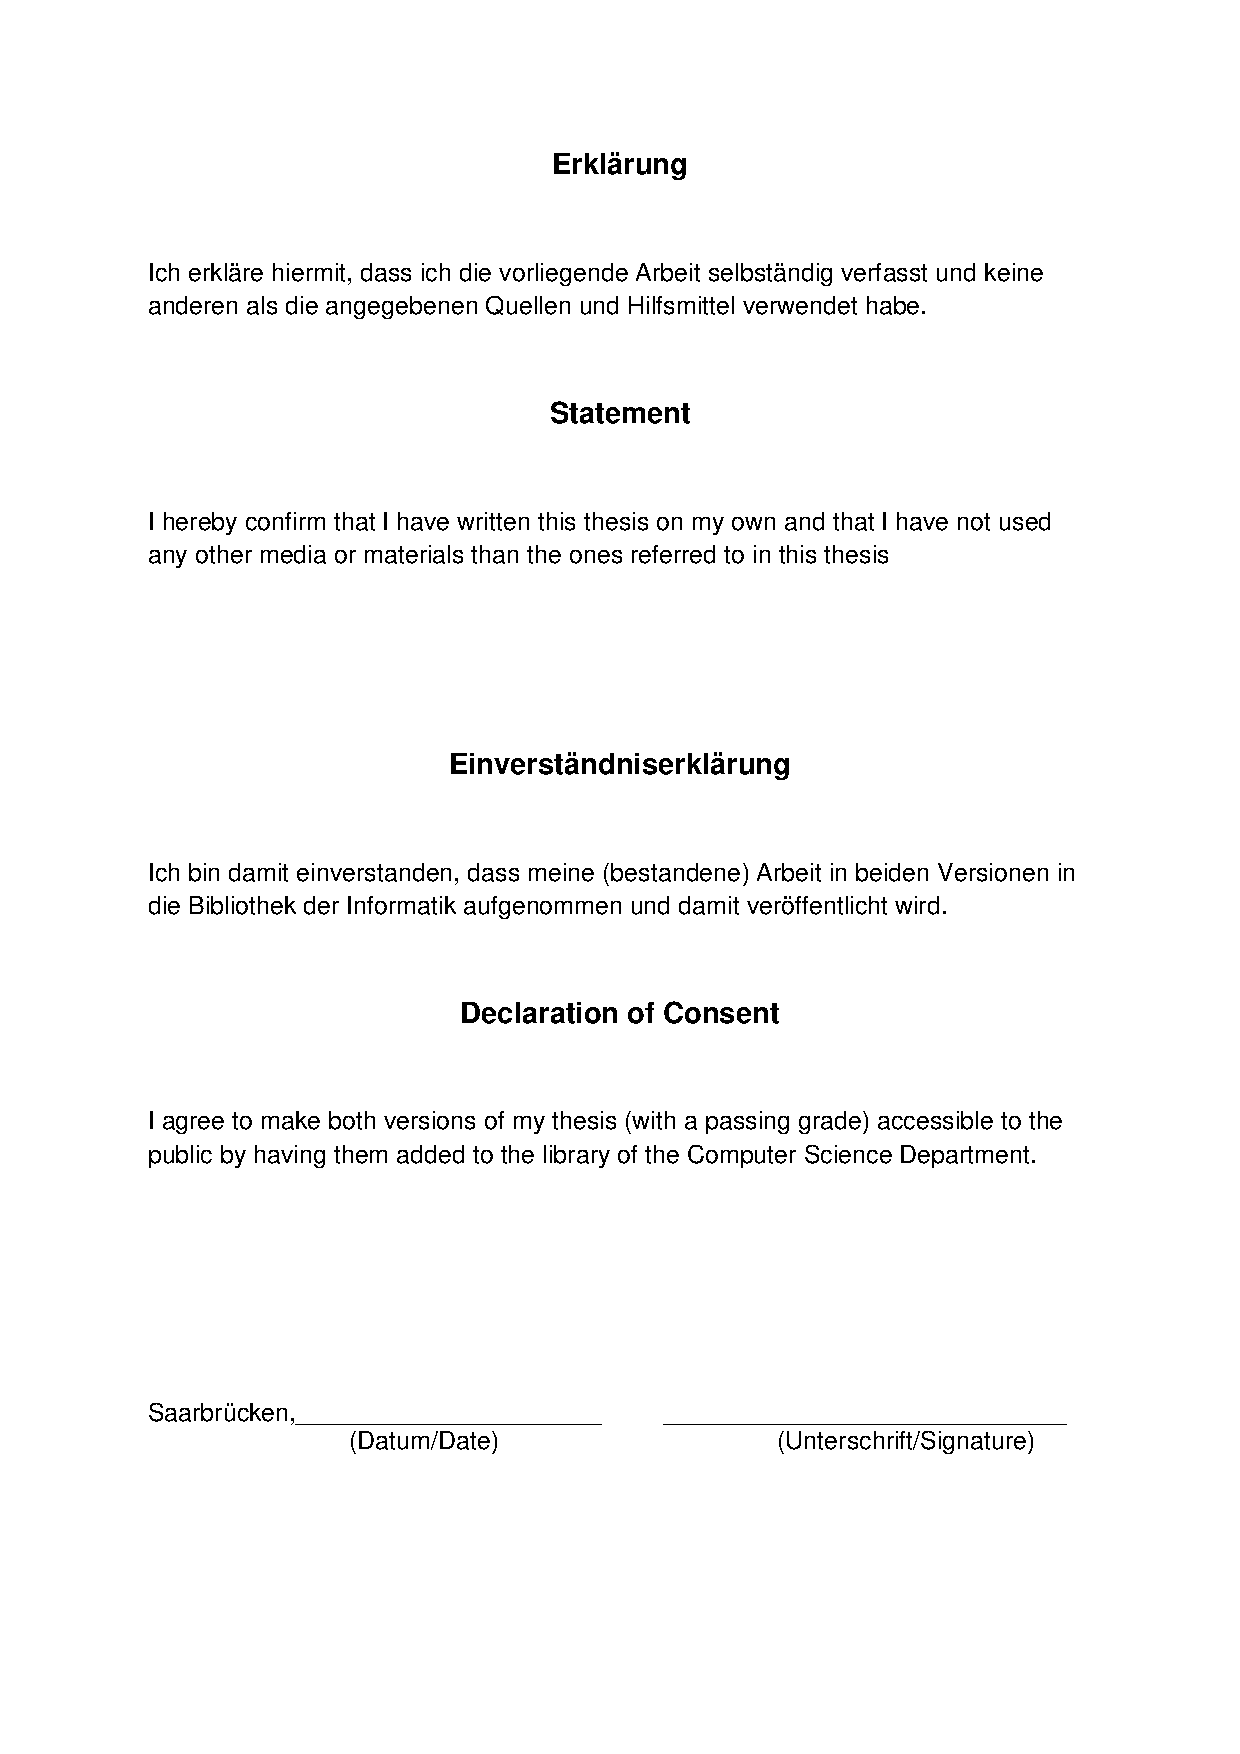
\includepdf{Images/statement.pdf}

\cleardoublepage

\begin{acknowledgements}
    \addchaptertocentry{\acknowledgementname}
    Firstly, I want to thank Prof.\ Dr.\ Joachim Weickert for his support and professional insight
    on the topic as well as for providing me with an interesting topic for my thesis. He always
    had an open ear for technical questions even despite the difficult situation that was
    Covid-19.\\
\\
    \noindent Naturally, I also want to thank Dr.\ Pascal Peter for accepting my
    request to be the second reviewer on such fairly short notice.\\
\\
    \noindent Moreover, I want to express my gratitude towards my friends and family for being 
    so supportive of me during the time of writing this thesis and for proof-reading early
    draft versions.\\
\\
    \noindent Last but certainly not least, I want to acknowledge my supervisor at work for 
    giving me the necessary time off to finish my thesis.
\end{acknowledgements}

%----------------------------------------------------------------------------------------
%   ABSTRACT PAGE
%----------------------------------------------------------------------------------------

\begin{abstract}
    \addchaptertocentry{\abstractname} 
    Over the last years, a new class of image compression codecs has been developed making use of
    novel inpainting techniques. These newly developed methods have been shown to have the
    potential to surpass common codecs like JPEG and JPEG2000. The idea behind them is to store a
    sparse subset of pixels and fill in the missing information with a digital image inpainting 
    algorithm. The challenge with such an approach is the choice of pixels that serve as the basis 
    to reconstruct the image. While the most successful ideas are based on stochastic or
    subdivision based methods, semantic approaches have barely been explored.
    In this thesis we build on results from a previous publication and further explore the potential 
    of reconstructing images by using only a set of corners from the image. We examine how 
    the accuracy of the corner detection influences the reconstruction quality and lastly introduce 
    additional procedures that aim to make the mask calculation a bit more robust with respect to
    the pixel density of the inpainting mask.
\end{abstract}

%----------------------------------------------------------------------------------------
%   ACKNOWLEDGEMENTS
%----------------------------------------------------------------------------------------

%----------------------------------------------------------------------------------------
%   LIST OF CONTENTS/FIGURES/TABLES PAGES
%----------------------------------------------------------------------------------------

\tableofcontents % Prints the main table of contents

%\listoffigures % Prints the list of figures

%\listoftables % Prints the list of tables

%----------------------------------------------------------------------------------------
%   thesis content - chapters
%----------------------------------------------------------------------------------------

% begin numeric (1,2,3...) page numbering
\mainmatter

\pagestyle{thesis} % Return the page headers back to the "thesis" style

% Include the chapters of the thesis as separate files from the Chapters folder
% Uncomment the lines as you write the chapters

\chapter{Introduction}\label{ch:Intro}
As technology evolves, the quality and resolution of digital images improve as well. But as the
quality increases so does the memory required to store the image on a hard drive. To counteract
this increase in disk space usage, people have tried to reduce the sizes of digital images a lot in the
last decades.\\
One of the most successful and probably most well known \textit{codecs}
is \textbf{JPEG}\cite{wallace91} and its lesser known but more advanced successor \textbf{JPEG 2000}\cite{jpeg2000}. Both are lossy image compression methods
known for fairly high compression rates while still providing a reasonable image quality.\\
For
higher compression rates however, the quality deteriorates pretty quickly and the infamous ``block
artifacts'' are being introduced. As a remedy, a new class of image compression methods based on
\textit{digital image inpainting} have been developed over the last
years~\cite{galic05, galic08, mainberger12, peloquin09, zimmer07, mainberger09, mainberger10, dong07, schmaltz09} that
aim to create better looking images for higher compression rates than JPEG and even JPEG2000. \\
Normally, inpainting methods are used to restore damaged paintings, remove objects from images,
etc., but by pushing these methods to their limits, they can also be used for image compression.
This can be accomplished by carefully selecting a very small subset of all pixels in the image, 
and then use such an inpainting method to restore the image from only the given data.
As one can imagine, selecting the right data is a fairly minute process and one has to carefully
select the pixels to keep. Even though there has been a lot of work done in this
area\cite{belhachmi09, schmaltz14, hoeltgen12}, the
selection can still be improved.\\
In the past, few methods explored how well corners/corner-like features do as candidates for
the inpainting process. In~\cite{zimmer07}, a method for image compression using corners was
proposed, but was not able to come close to the performance of JPEG. However, this method did not
explore its full potential. One of the main points of criticism is, that the corner localisation
was not accurate enough, or rather the inaccuracies were not accounted for in the mask
selection\cite{conversation}. This is why I want to improve on this approach and try to tap into
its unexplored potential.\\

\subsection*{Goal}\label{ssub:Goal}

The goal of this thesis is two-fold:
First, I want to explore how the inaccuracies in the corner localisation can be properly accounted
for in the mask creation. This includes finding out how large the corner region disks have to be to
counteract the inaccuracy introduced during the detection phase.\\
Secondly, I want to introduce some additional procedures to improve the selection of corner regions
and make it a bit more robust with respect to the pixel density in the final mask, as it is fairly
important to reliably produce masks containing only a certain percentage of pixels if one wants to
use this approach for image compression.
One of the biggest factors that I had to consider was, that corners and similar features can be quite 
rare in images, severely limiting the amount of candidates one can choose from, especially compared to
approaches like \cite{schmaltz09, hoeltgen12}. 
I will cover these procedures in \ref{sec:Contribution} while the first goal will be covered in
\ref{sec:ParameterSelection}.

\chapter{Related Work}\label{ch:RelatedWork}
In this chapter I will discuss some publications that are closely related to my thesis. 
In the first part I will give a short recap on the evolution of PDE-based image compression from
its first mention to today to give more context about the overall field of research this thesis 
resides in.
Afterwards, I am going to adress some publications in the more narrow field of image compression
using semantic features like edges and corners, one of which is subject to improvement that is 
discussed in this thesis.
\section{PDE-based Image Compression}
In recent years, a new image codec relying on an inpainting process based on solving partial
differential equations was developed as an alternative to JPEG and JPEG2000. 
The core idea is to compress the image by selecting a set of pixels that serves as the basis for the 
inpainting process. 
This inpainting process is defined by a partial differential equation that is solved iteratively during 
the reconstruction phase.\\
In 2005, Galić et al.~\cite{galic05}\ first introduced an image compression method using nonlinear
anisotropic diffusion as a serious alternative to more classical approaches like JPEG.\@
In this work, the authors showed the inpainting capabilities of a diffusion process known as edge-enhancing
diffusion (or short EED), which has since then established itself as the prime choice for PDE-based image
compression. The approach they presented relies on efficiently storing a pixel mask that is later
on used to reconstruct the image by filling in the missing regions using the aforementioned process
of edge-enhancing diffusion and lays the groundwork for later publications building on the codec
defined therein. \\
As already mentioned, the codec relies on computing a pixel mask from the original image. However,
this process is a balancing act. On one hand, one wants to get a mask that yields a perfect
or at least close to perfect reconstruction of the original image but on the other hand, one 
also wants to create a mask that
can be encoded and stored efficiently, i.e.\ using the smallest amount of \textit{bits-per-pixel
(bpp)} possible. This step of mask computation is still topic of ongoing research which gives a
good idea of the difficulty of this problem.\\
In the initial codec, also called the \textbf{BTTC-EED} codec, the mask was
computed by means of an adaptive sparsification scheme relying on B-tree triangular coding (BTTC)
that was already introduced by Distasi et al.~\cite{distasi97} back in 1997. This fairly simple
approach iteratively subdivides the image diagonally if the error of the reconstruction of the image using only
the corner points of the subdivision exceeds an a priori defined threshold. In this version, the
reconstruction is approximated by a simple linear interpolation inside the triangle. The efficiency
of constructing a mask using BTTC lies in the binary tree structure of the subdivision that can be encoded extremely
efficiently by a simple binary string. Furthermore, grey values are encoded using a straight
forward entropy coding method, i.e.\ Huffman coding~\cite{huffman} in this case.
With this approach, they were already able to outperform JPEG visually for high
compression rates and comic-style images~\cite{galic05}.\\
\\
In~\cite{schmaltz09}, this approach was further improved by the addition of several optimisation
steps. They found that by replacing the triangular subdivision by an adaptive rectangular
subdivision procedure, the quality of the reconstructed images could be improved. Furthermore,
instead of the simple Huffman encoding, they switched to a more advanced entropy coding standard
called \textit{PAQ}~\cite{paq}. \\
Additional optimisations they introduced include a brightness rescaling
step, a reconstruction parameter optimisation step and finally a step they called `interpolation
swapping'.
In the brightness rescaling step, the grey value range of mask pixels was adjusted to use up the 
full range in order to reduce quantisation artifacts.
The parameter optimisation aims to find an optimal diffusivity parameter for the diffusion step in
the reconstruction phase. This optimised parameter is then also stored in the compressed image.
By including this step, they were able to cut the reconstruction error in half.\\
Last but not least, they introduced a process called `interpolation swapping' that is performed
after the decompression phase. In this procedure, in the reconstructed image, the roles of mask
pixels and inpainted pixels are reversed for a final diffusion step to smooth out any artifacts
that may occur on the boundary between known and unknown pixels during the decompression phase.\\
With all these additions, this new codec called \textbf{R-EED} is able to actually outperform the
successor to the JPEG codec, namely JPEG2000 even for high compression rates.
\begin{figure}[ht]
    \centering
    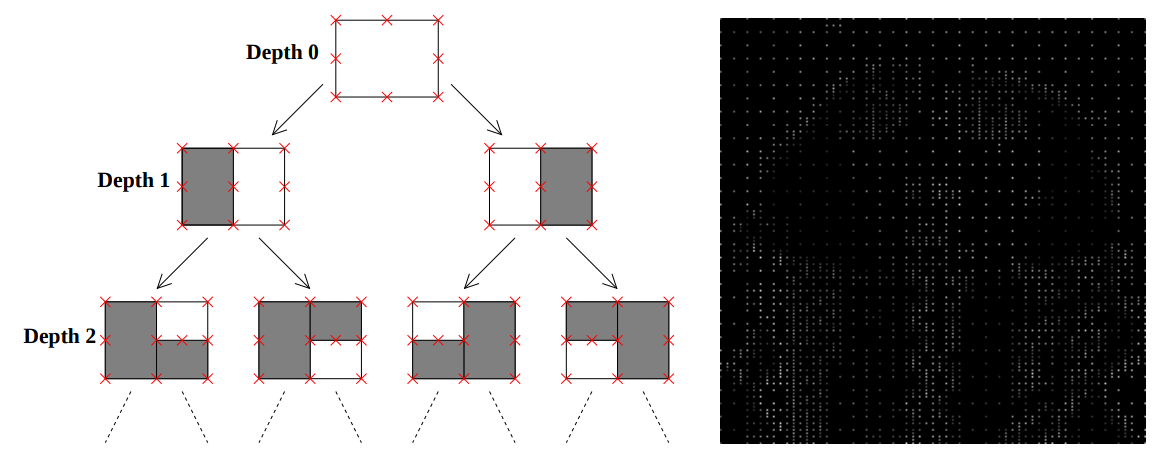
\includegraphics[width=0.8\linewidth]{../Images/tree_trui.png}
    \caption{Examples for rectangular subdivision in the R-EED codec~\cite{schmaltz09}.}
\end{figure}
In~\cite{hoeltgen12}, an alternative approach to the rectangular subdivision used in
~\cite{schmaltz09} was proposed. They considered two different methods. First, they used the results
from~\cite{belhachmi09} to derive an \textit{analytical approach} by calculating the \textit{Laplacian of a
Gaussian} $\vert \Delta f \vert^s$ for some exponent $s>0$ and then apply electrostatic 
halftoning~\cite{electrostatic} in order to get a binary point mask.\\
The second method they proposed is called \textit{probabilistic sparsification}. It works by
iteratively selecting a set percentage of pixels from the original image into the mask,
reconstructing the image using the same inpainting operator as in the decompression step, then
calculating the reconstruction error for each pixel in the inpainting mask and then throwing out
the pixels with the largest reconstruction error. This is repeated until a predefined pixel
density in the mask is reached. However, the authors stated that this method is not guaranteed to
give an optimal solution because of its greedy nature. To improve the mask they derived in the
earlier step, they introduced the so called \textit{nonlocal pixel exchange}. It aims to solve the
problem that the greediness of the probabilistic sparsification poses, more specifically that
pixels that were removed once are not considered again at a later point in time even though they
could possibly positively influence the quality of the final mask.\\
The nonlocal pixel exchange randomly selects a subset of non-mask pixels, from which the pixel with
the largest reconstruction error is put in the mask in exchange for a random mask pixel.
If the overall reconstruction quality improves with the new mask, the mask is updated to the new
mask and serves as the initial mask for the next iteration step. If the quality deteriorates with
the new mask, the change is undone and the procedure continued.
The mask resulting from this process can only be better than the previous one by construction of
the algorithm~\cite{hoeltgen12}.
Finally, they proposed several algorithms for \textit{tonal optimisation}, i.e.\ grey value
optimisation by means of a linear least squares optimisation problem. They showed some important
mathematical properties like the uniqueness and existence of a solution for this problem and
came up with a numerical algorithm to solve the linear system of equations arising for this
optimisation problem.
Using all these optimisations, they were able to cut down the reconstruction error in terms of the
mean squared error by a significant portion and achieve a quality that has not been reached before 
with similar PDE based inpainting approaches for the same mask density.

\section{Image Features In Image Reconstruction}
Features such as edges and corners are very important in the field of image processing as they
provide almost all of the semantics of an image~\cite{marr82}. Therefore, feature detection has been a staple in
this field for a long time. Actually, corner and edge detection algorithms such as the ones by John Canny
and Chris Harris~\cite{harris88, canny86} are still used today. 
Despite their semantical importance, edges and corners have not had that much impact on image
compression so far.\\
\\
In 2007, Zimmer introduced a new approach using corners to compute inpainting masks for
PDE-based image compression~\cite{zimmer07}. In their approach, they used a simple corner detection method to
sample a set of the most important corners. The inpainting mask was then obtained by storing the
8-neighbourhood around each corner. In the reconstruction or inpainting phase they used a method
following the idea proposed by Bertalmio et al.~\cite{bertalmio00}. Instead of just using pure EED to
inpaint the image, they interleaved edge-enhancing diffusion with mean curvature motion in order to
improve the inpainting in regions with sparser inpainting domains. \\
Even though their codec was
not able to compete with widely used codecs like JPEG and JPEG2000, they proved that corners are
indeed useful for PDE based inpainting. They found the largest disadvantages to be the sparsity of
corners in images. The reasoning behind this is that because of the sparsity of corners in an
image, one has to either invest in a very sophisticated and complex inpainting mechanism to fill in
the large areas between the few detected corners \textit{or} adjust the corner detector to be more
`fuzzy'. On one hand, this leads to a denser mask and hence better results reconstruction-wise 
but on the other also creates suboptimal masks with respect to compression. Due to the fuzzy nature of the
corner detector, flat or homogeneous areas are classified as corners and therefore kept in the
mask, even though these regions could have easily been filled in by even a simple inpainting
process like linear diffusion. \\
To improve on their work, they suggested to touch on the parameter
selection for the corner detector, especially the selection of both the cornerness threshold and
integration scale used in the computation of the structure tensor since these heavily influence the
amount and quality of corners that are detected. \\
The main point of criticism for this approach is that the inaccuracy of the corner 
detector was not accounted for in the selection of the mask
pixels~\cite{conversation}. Their method of limiting the amount of mask pixels by adjusting the integration scale leads
to a fairly inaccurate localisation of the corners. The cause for this will be discussed in
a later section.
Since only a small neighbourhood of pixels around each estimated corner
location was kept, the likelihood that the actual corner is not included in the final mask
increases the larger the integration scale is chosen, as we will see in Chapter~\ref{ch:Implementation}, 
where I will also adress how to approach this problem and provide a possible solution.\\
\\
In~\cite{mainberger09, mainberger10}, the authors implemented a diffusion based reconstruction
using mainly edges as the inpainting mask. For the mask construction they used the Marr-Hildreth
edge detector~\cite{marr80} combined with \textit{hysteresis thresholding} as proposed by
Canny~\cite{canny86}.
However, they stated that they were not locked in on the Marr-Hildreth edge detector and that
others such as the classical Canny edge detector could also be used, especially for images that
contain a larger amount of blurry edges. The addition of hysteresis thresholding yielded closed and
well localised contours which they encoded using the lossless \textit{JBIG} encoding~\cite{jbig}.
To reconstruct the image from the stored contours, they used a simple linear diffusion approach
which, in this case, was good enough. For cartoon-like images, they could beat the quality of
JPEG and even the more sophisticated JPEG2000 in terms of the PSNR (peak signal to noise ratio) of the reconstructed image to the
original one. In the follow-up publication from the same authors in 2010 they introduced some 
optimisations such as different
entropy coders for the edge locations as well as an optimised method of storing the grey
values of the mask pixels. Another improvement was the use of an advanced method for solving the
linear systems arising from the inpainting problem. In contrast to the earlier publications a fast
\textit{full multigrid scheme} was implemented to speed up the decoding phase significantly to 
a point where the codec is now realtime capable.\\
\\
In~\cite{peter15}, region of interest (ROI) coding was first introduced for the R-EED codec. Previously,
it was not possible to specify certain regions of an image to be reconstructed with higher detail.
With this new contribution, they allowed the user to specify a weighting mask that is used during
the mask construction phase to adapt the mask in such a way that the specified regions would have a
denser mask than other regions. This is expecially useful in medical imaging, where some regions of
an image, e.g.\ in a CT scan of a brain region, need to be reconstructed exactly in order to prevent
false diagnoses. \\
ROI coding was not the only contribution in this publication. The authors also proposed
\textit{progressive modes} for the R-EED codec to be able to compete better with widely available codecs.
Progressive modes allow an image to be displayed in a coarse manner, e.g.\ when shown on a website
that has not fully loaded the image data yet, and gradually refine the representation as more data
becomes available. Last but certainly not least, they showed that their PDE-based codec is also
capable of realtime video decoding and playback which sets a milestone in proving the
\textit{suitability of R-EED for real-world applications}~\cite{peter15}. In their words, this
publication, or rather the extensions presented therein, mark the first step of an evolution of
PDE-based compression codecs from the proof-of-concept stage to fully grown codecs with relevance
for practical applications~\cite{peter15}.\\
\\
In~\cite{kanters05}, a method is presented that uses extrema and saddle points in the Gaussian
scale space of an image as a basis for reconstruction using a linear reconstruction scheme proposed
in~\cite{janssen05}.\\
In~\cite{weinzaepfel11}, the authors explore the reconstruction of an image using only its local
descriptors. They use a classical image indexing software to retrieve descriptors like
SIFT~\cite{sift}, then query an image database to find patches that are similar to these descriptors
retrieved from the image. These patches are then transformed to fit the geometry in the original
image and stitched together afterwards in a seamless fashion.

\section{Outline}
So far, we have reviewed some of the work that is closely related to my work and 
motivated the goal that I am tring to achieve.
To explain what exactly was done in order to achieve this goal, we first have to go over some of the
theoretical background. I will introduce basic concepts from
calculus and linear algebra (\ref{sec:Basics}) as well as some more advanced topics
like the structure tensor (\ref{sec:Structure}), diffusion processes (\ref{sec:Diffusion}) and
digital image inpainting (\ref{sec:Inpainting}).\\
In Chapter~\ref{ch:Implementation}, I will then talk about the technical details of the  
implementation, for example the discretisation used to implement the theoretical ideas from 
the previous chapter (\ref{sec:Discretisation}). 
Furthermore, I will describe the shortcomings of the approach described in~\cite{zimmer07} in more
detail and discuss a method to address these issues. In this chapter, I will also present some
additional procedures that I implemented in order to improve the selection of mask pixels. \\
Afterwards, I am going to review the experiments that were performed in order to evaluate the
approach and show some examples.\\
Last but not least in Chapter~\ref{ch:Conclusion}, I conclude the work, discuss the strengths
and shortcomings of my approach and how it could be improved in future research.

\newcommand{\TODO}[1]{\ \\ \textbf{\textcolor{red}{!! #1 !!}}\\}
\chapter{Theoretical background}\label{ch:Theory}
%%%%%%%%%%%%%%%%%%%%%%%%%%%%%%%%%%%%%%%%%%  Basics %%%%%%%%%%%%%%%%%%%%%%%%%%%%%%%%%%%%%%%%%%%%
\section{Basics}\label{sec:Basics}
The concepts used in this thesis require some prior knowledge about basic calculus and linear
algebra as well as some more advanced topics that will be introduced in the following sections.
But before introducing corner detection and diffusion, we have to first define what an image is
mathematically.\\
A \textit{grey value image} is defined as a function $f: \Omega \rightarrow \mathbb{R}$ where
$\Omega \subset \mathbb{R}^2$ is a rectangular subset of $\mathbb{R}^2$ of size $n_x\times n_y$,
wheras a
\textit{colour image} is defined as a vector-valued function $f: \Omega \rightarrow \mathbb{R}^3$.
For the sake of simplicity, we will focus on grey value images as most of the results can easily be
transferred to vector-valued images.\\
\textbf{Notation:} Instead of writing $(x, y)$, I will use $\boldsymbol x := (x, y)$ most of the
time, as it makes most equations and definitions more readable. Furthermore, lowercase bold letters will denote vectors and uppercase bold letters will
denote matrices.
\subsection{Image gradient}
One of the most important operations on functions in image processing is \textit{partial
    differentiation}.
The partial derivative of an image $f: \Omega \rightarrow [0, 255]$ in $x$-direction is herein denoted as $f_x$ or
synonymously as $\partial_x f$ and defined as
\begin{equation}
    f_x(x, y) = \partial_x f (x, y) = \frac{\partial f}{\partial x} (x, y) := \lim_{h \to 0}\frac{f(x+h, y) -f(x, y)}{h} 
\end{equation}
The \textit{gradient} of an image $f$ is the vector containing both partial image derivatives.
In multivariable calculus, the gradient of a function is an important tool to find the (both local
and global) extrema of a function similar to the first derivative for a function with a single
variable.
\begin{equation}
    \textbf{grad}(f) = \boldsymbol\nabla f := \left(f_x, f_y\right)^\top
\end{equation}
The gradient always points in the direction of the steepest ascent/descent, it is the tangent
vector to the surface at the given location\cite{mfi3}.
Note that the gradient of a function is a vector-valued function and not a vector.

\subsection{Convolution}
Another operation from calculus that we will need is the \textit{convolution operator}.\\
\begin{equation}
    (f * g)(\boldsymbol x) := \int\limits_{\mathbb{R}^2} f(\boldsymbol x-\boldsymbol y)g(\boldsymbol y)d\boldsymbol y\label{eq:2DConv}
\end{equation}
Convolution is especially useful in image and signal processing to design so called linear filters
such as a moving average or smoothing operation\cite{ipcv19-02,dic18-02}. As a matter of fact, in a later
section we will need the convolution as a tool to smooth our image to reduce noise artifacts. To
achieve this, we will use a \textit{Gaussian convolution}, i.e.\ a convolution with a
\textit{Gaussian kernel} which is basically just a two-dimensional Gaussian function with a certain
standard deviation\cite{ipcv19-02}:
\begin{equation}
    K_\sigma (\boldsymbol x) := \frac{1}{2\pi\sigma^2}\exp\left(\frac{-\lVert\boldsymbol
            x\rVert_2^2}{2\sigma^2}\right)
\end{equation}
where $\lVert \cdot \rVert_2$ denotes the \textit{Euclidean norm}.
For the rest of this thesis, an image $f$ convolved with a Gaussian with standard deviation $\sigma$
will be denoted by \[f_\sigma := K_\sigma * f\]
Note that because of the symmetry of the
convolution, it would have been perfectly fine to write it as $f * K_\sigma$.

%%%%%%%%%%%%%%%%%%%%%%%%%%%%%%%%%%%%%%  Structure Tensor %%%%%%%%%%%%%%%%%%%%%%%%%%%%%%%%%%%%%%
\section{The Structure Tensor}\label{sec:Structure}
For some applications only the gradient of an image does not give us enough information. The
gradient on its own is mostly just used as an edge detector, hence we need to come up with
something else for e.g.\ corner detection\cite{ipcv19-13}. One option is the so called \textit{structure tensor}, a
matrix that contains information about the surrounding region at a specific position. With the
structure tensor, or rather its eigenvalues (cf.~\ref{sub:Corner}), one is able to
distinguish between flat regions, edges and corners.

\subsection{Definition}
\TODO{Reconsider the definition, maybe rewrite this paragraph later}
The structure tensor is defined as a matrix whose eigenvectors tell us the direction of
both the largest and smallest grey value change. Mathematically, we can model this
as an optimisation problem:\\
Let $u$ be a grey value image.
We want to find a unit vector $\mathbf{n} \in \mathbb{R}^2$ that is `most parallel' or `most orthogonal' to the
gradient $\boldsymbol\nabla u$ within a circle of radius $\rho > 0$, i.e. one wants to optimise the
function
\begin{align}
    E(\mathbf{n}) &= \int\limits_{B_\rho(\boldsymbol x)} \left(\mathbf{n}^\top\boldsymbol\nabla
        u\right)^2d\boldsymbol x'\\
    &= \mathbf{n}^\top \left(\int\limits_{B_\rho(\boldsymbol x)} \boldsymbol\nabla u \boldsymbol\nabla
        u^\top d\boldsymbol x' \right) \mathbf{n}\label{eq:QuadForm}
\end{align}
This function is also called the \textit{local autocorrelation function/local average
    contrast}\cite{harris88, ipcv19-13}.
Since~\eqref{eq:QuadForm} is a quadratic form of the matrix
\[M_\rho(\boldsymbol\nabla u) := \int\limits_{B_\rho(\boldsymbol x)} \boldsymbol\nabla u \boldsymbol\nabla
    u^\top d\boldsymbol x'\]
such an optimal unit vector is by definition also the eigenvector to the smallest/largest
eigenvalue of $M_\rho(\boldsymbol\nabla u)$\cite{ipcv19-13}.
The matrix $M_\rho(\boldsymbol\nabla u)$ can also be seen as a component-wise convolution with the indicator
function
\[b_\rho(\boldsymbol x) = \begin{cases} 1 & \lVert \boldsymbol x\rVert_2^2 \leq \rho^2\\ 0 & \text{else} \end{cases}\]
However, as the author stated in \cite{harris88}, using this \textit{binary window function} leads
to a noisy response and they therefore suggest using a \textit{Gaussian window function} with standard
deviation $\rho$. This parameter is also
called the \textit{integration scale} and determines how localised the structure information
is\cite{ipcv19-13}.
This ultimately leads to the definition
\begin{equation}
    \mathbf{J}_\rho(\boldsymbol\nabla u) := K_\rho * (\boldsymbol\nabla u\boldsymbol\nabla u^\top)
\end{equation}
It is important to state that almost always, one uses a smoothed or \textit{regularised} image instead of the
original unregularised form in order to reduce numeric instabilities caused by
differentiation\cite{ipcv19-12}. The definition then becomes
\begin{equation}
    \mathbf{J}_\rho(\boldsymbol\nabla u_\sigma) := K_\rho * (\boldsymbol\nabla u_\sigma\boldsymbol\nabla
    u_\sigma^\top)\label{def:StructTensor}
\end{equation}
To keep things simpler, I will omit the brackets and just simply use $\mathbf{J}_\rho$ as the
structure tensor.\\
\subsection{Usage in Corner Detection}\label{sub:Corner}
The structure tensor is a symmetric matrix and thus possesses orthonormal eigenvectors $\boldsymbol v_1,
\boldsymbol v_2$ with real-valued eigenvalues $\lambda_1, \lambda_2 \geq 0$. \cite{ipcv19-13} As
mentioned in the preface to this section, we can use these eigenvalues to distinguish between
corners, edges and flat regions as seen in figure \ref{fig:Structure}.
In total, we have to deal with 3 different cases:
\begin{enumerate}
    \item $\lambda_1, \lambda_2$ are both small $\rightarrow$ flat region
    \item one of the eigenvalues is significantly larger than the other one $\rightarrow$ edge
    \item both eigenvalues are significantly larger than 0 $\rightarrow$ corner
\end{enumerate}
If one looks at the eigenvalues as indicators of how much the grey value shifts in the
corresponding
direction, then the classification makes perfect sense. If both eigenvalues are small, then the
grey value does not shift much in either direction, thus the area does not contain any features.
In the case that one is much larger than the other one, there is an edge in direction of the
eigenvector of the larger value since the largest grey value shift is in exactly this direction.
For the last case it should be obvious why this refers to a corner region. When both eigenvalues
are large, there is a large grey value shift in either direction, therefore there has to be a
corner.\\
\begin{figure}[h]
    \centering
    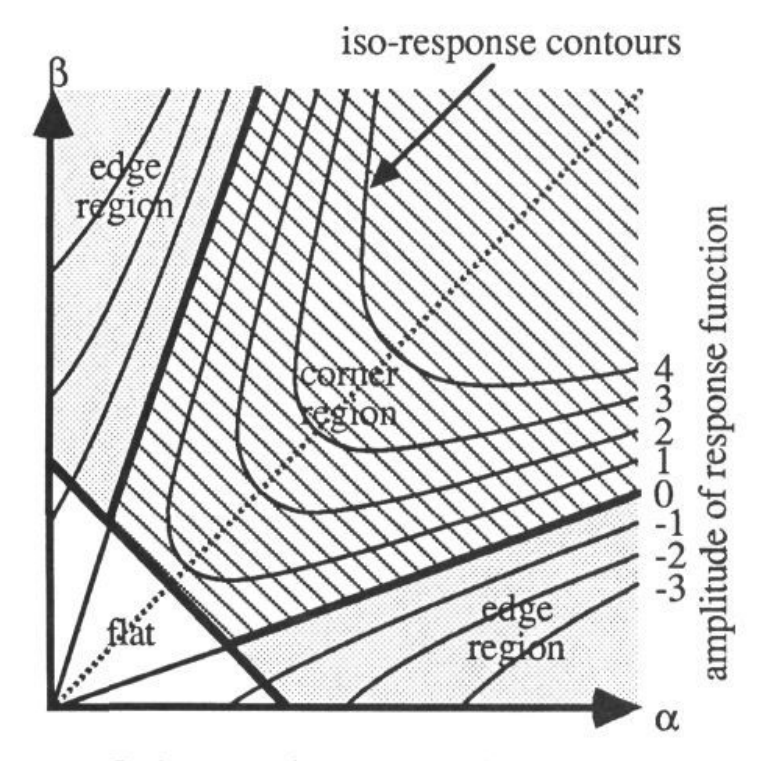
\includegraphics[width=0.6\linewidth]{../Images/structure_tensor.png}
    \caption{Visualisation of distinction of image features using the eigenvalues of the structure
        tensor. $\alpha, \beta$ are equivalent to the eigenvalues $\lambda_1, \lambda_2$. Source: \cite{harris88}}\label{fig:Structure}
\end{figure}
There are several approaches to find out which case applies at the current position. The biggest
challenge here is to differentiate between edges and corners, i.e. we have to find out whether both
eigenvalues are meaningfully larger than 0 and if one is larger than the other.\\
The most intuitive approach is the one by Tomasi and Kanade, sometimes also called Shi-Tomasi
corner detector. It simply compares the smaller eigenvalue against some artificial
threshold. The set of local maxima is then the set of corners for the image\cite{shitomasi94}.
However, this approach requires to compute both eigenvalues and can thus be fairly expensive.\\
\TODO{Find sources for Rohr and Förstner}
A cheaper approach would be to either threshold the trace \[tr(\mathbf{J}_\rho) := j_{1, 1} + j_{2,
        2} = \lambda_1 + \lambda_2\] as proposed by Rohr, 1987 or the determinant \[det(\mathbf{J}_\rho) := j_{1, 1}j_{2, 2} -
    j_{1, 2}^2 = \lambda_1\lambda_2\] as proposed by Harris and F\"orstner, 1988 and 1986
respectively\cite{harris88}. Both of these approaches do not need to explicitly compute the eigenvalues of
the structure tensor and are thus not as computationally invested. Another difference between both 
approaches is that the first one requires the trace by itself to be a local maximum whereas in the
second approach, $(det(\mathbf{J}_\rho))/(tr(\mathbf{J}_\rho))$ needs to be a local maximum.\\

For the detection of relevant corners in the data selection phase, I mainly used the approach of F\"orstner/Harris as well as
the approach of Rohr even though the Tomasi-Kanade approach was an option and has also been
tested as we will see later in chapter \ref{ch:Experiments}. However, it has not proven as successful
as the other two methods during the initial testing phase.
%%%%%%%%%%%%%%%%%%%%%%%%%%%%%%%%%%%%%  Diffusion %%%%%%%%%%%%%%%%%%%%%%%%%%%%%%%%%%%%%%%%%%%%%%
\section{Diffusion}\label{sec:Diffusion}
The concept of diffusion is omnipresent in the physical world. It describes, in the broadest sense
possible, how particles distribute in a certain medium. This could be anything from heat in air to
ink in water. But this is not its only use. It is applicable in many more fields ranging from
natural sciences to finance and economics. In this chapter, we will see how diffusion applies to
image processing and what benefits we gain from it. Furthermore, I will go over some basic ideas to
introduce diffusion mathematically and subsequently explain different types of diffusion commonly
found and used in image processing.
\subsection{A short note on scale spaces}
Before we begin to talk about diffusion, I will use this opportunity to shortly introduce scale
spaces and explain how they are useful to diffusion processes in image processing and image
processing in general.\\
A scale space is generally defined as a family of images with a time parameter $t$ that become
increasingly `simpler' as $t \to \infty$. The point of a structure like this is, that certain image
features do only exist at a specific scale or a range of scales and that it is therefore beneficial
to the understanding of an image to basically have a hierarchy of features.\\
Mathematically, a scale
space needs to meet certain requirements like the semi-group property, maximum-minimum principles
and others.
A full explanation of all the scale space requirements would be beyond the scope of this thesis
and is frankly not needed to understand the following sections.\\
To embed an image $f:\mathbb{R}^2 \rightarrow \mathbb{R}$ in a scale space, we need a smoothing
operator $T$ that is applied iteratively to the image. One such an operation is the Gaussian
convolution: 
\begin{equation}
    T_tf := K_{\sqrt{2t}} * f
\end{equation}
This operation spans the \textit{Gaussian scale space}, one of if not the the oldest and best
understood scale space. In the western world, it was first mentioned by Witkin et
al.\cite{witkin84} 1984, but as was later found out, researchers in Japan already proposed it in
1963\cite{weickert-ishikawa}.\\
Scale spaces as a tool are very important to diffusion filtering, since diffusion is an iterative
process and as such benefits from the notion of a scale spaces. Embedding an image in such a scale
space allows us to develop a theory of evolving the image over time as we will see in the next
sections, where I will first show the basic idea behind the general diffusion equation and
subsequently introduce different types of diffusion important to image processing.
To avoid confusion we define the gradient for scale spaces as the \textit{spatial gradient} 
\begin{equation}
    \boldsymbol\nabla u(x, y, t) = \begin{pmatrix}
        \partial_x u(x, y, t)\\
        \partial_y u(x, y, t)
    \end{pmatrix} 
\end{equation}
instead of the spatiotemporal gradient.

\subsection{Mathematical background}
To get a glimpse of the basic idea of diffusion, we have to take a small dive into the world of
physics.
As mentioned in the introduction to this section, diffusion is used to describe processes of
particle or concentration distribution. The differences in concentration are evened out by a flow
or \textit{flux} that is aimed from high concentration areas to areas with low concentration. This
principle is stated by \textit{Fick's law}\eqref{eq:Fick} (hence this type of diffusion is called \textit{Fickian
diffusion}):
\begin{equation}
    \boldsymbol j = -\boldsymbol D\cdot\boldsymbol\nabla u\label{eq:Fick}
\end{equation}
Here, the flow from high to low concentration areas is modelled by a flow whose direction is
proportional to the inverse direction of the largest change in concentration, i.e. the gradient.
While most of the time, the gradient determines the direction of the flux, the so called
\textit{diffusion tensor} $\boldsymbol D$ determines its strength. In general, this diffusion
tensor is defined as a
$2\times2$ positive definite matrix, but as we will see later, it can be reduced to a scalar 
valued function in more simple cases.
In more complex cases, also called \textit{anisotropic}, the diffusion tensor can also adjust the
direction of the flow. We will see how this works in the section about \textit{nonlinear
anisotropic diffusion}.\\
Another important principle for diffusion is the conservation of mass, since mass cannot be created
out of thin air and similarly cannot simply vanish.
This principle is given by the equation
\begin{equation}
    \partial_t u = - \textnormal{div}(\boldsymbol j)\label{eq:Conservation}
\end{equation}
where $u: \Omega \times [0, \infty) \rightarrow \mathbb{R}$ is a function of time and space and div
is the \textit{divergence operator}
\[\textnormal{div}(\boldsymbol j) := \partial_x j_1 + \partial_y j_2\]
\begin{figure}[h]
    \centering
    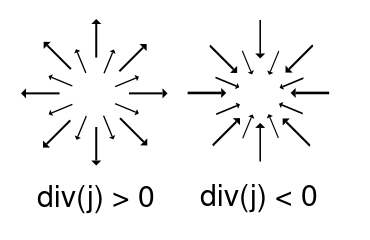
\includegraphics[width=0.5\linewidth]{../Images/divergence2.png}
    \caption{Visualisation of the divergence operator. Original image \cite{img-divergence}
    edited with GIMP}\label{fig:Divergence}
\end{figure}
In simple terms, the divergence of the flux measures whether the concentration at the current
location diverges, i.e. diffuses away from the current location, or converges, i.e. moves in
towards the current location.
Together, equations~\eqref{eq:Fick} and \eqref{eq:Conservation} then form the general \textit{diffusion
    equation}\cite{dic18-02, weickert96}
\begin{equation}
    \partial_t u = \textnormal{div}(\boldsymbol D\cdot\boldsymbol\nabla u)\label{eq:Diffusion}
\end{equation}
%To solve this equation, it is embedded in the initial value problem
%\begin{align}
    %&\partial_t u = \textnormal{div}(\boldsymbol D\boldsymbol\nabla u)&\textnormal{on}\ 
    %\Omega\times[0, \infty)\\
    %&u(\boldsymbol x, 0) = f(\boldsymbol x)&\textnormal{on}\ \Omega\\
    %&\boldsymbol n^\top \boldsymbol D\boldsymbol\nabla u = 0&\textnormal{on}\ 
    %\partial\Omega\times[0, \infty)
%\end{align}
The solution to this equation can be interpreted as an image embedded in a scale space with the
evolution time as the scale parameter. To get different scale spaces ergo different diffusion
processes, one can alter the diffusion tensor in certain ways.
In the following, we will see how different diffusion processes are characterized and what they are
generally most useful for in image processing.

\subsubsection*{Linear isotropic diffusion}
In this first and simplest case, the diffusion tensor is replaced by a constant diffusivity
resulting in equal smoothing all across the image. The constant diffusivity can also be expressed
as the identity matrix $\boldsymbol I$ which simplifies the diffusion equation to the 2D\textit{
heat equation}
\begin{equation}
    \partial_t u = \Delta u = \textnormal{div}(\boldsymbol\nabla u)
\end{equation}
which can be solved analytically. The solution to this equation has proven to be equivalent to
a Gaussian convolution, thus this type of diffusion also produces a Gaussian scale space.\\
Obviously, homogeneous smoothing is not very useful if one wants to create a filter that is able to
enhance edges. Still, it is the best understood and oldest scale space and used for many
applications in image processing. One example is optical character recognition.
However, to achieve edge enhancing properties, we need to look into nonlinear methods.

\subsubsection*{Nonlinear isotropic diffusion}
Previously, we replaced the diffusion tensor by the identity matrix, which resulted in the same
amount of smoothing at every location.
To get spatially varying smoothing, we have to introduce a \textit{diffusivity} function that
depends continuously on the input image. 
\begin{align}
    \boldsymbol D &= g(\lVert\boldsymbol\nabla u\rVert_2^2)\boldsymbol I\\
    \Rightarrow \partial_t u & = \textnormal{div}(g(\lVert\boldsymbol\nabla u\rVert_2^2)\boldsymbol\nabla u)
\end{align}
The diffusivity function determines how much the image should be smoothed at the current location.
The most well known choice for a diffusivity function was proposed by Perona and Malik 
\cite{perona-malik}
\begin{equation}
    g(s^2) = \frac{1}{1 + s^2/\lambda^2}\label{def:Diffusivity}
\end{equation}
The interesting part about this diffusivity function is that it distinguishes between edges and
non-edges or flat areas according to the \textit{contrast parameter} $\lambda$ using the gradient
magnitude $\lVert\boldsymbol\nabla u\rVert_2^2$ as a \textit{fuzzy edge detector}\cite{dic18-04}. An important part
to understanding why this leads to an edge enhancing effect is the flux function
arising from this specific diffusivity. In general, the flux function is simply defined as 
\begin{equation}
    \Phi(s) = sg(s^2)
\end{equation}
which in this particular case comes down to
\begin{equation}
    \Phi(s) =\frac{s}{1 + s^2/\lambda^2}\label{def:Flux}
\end{equation}
\begin{figure}
    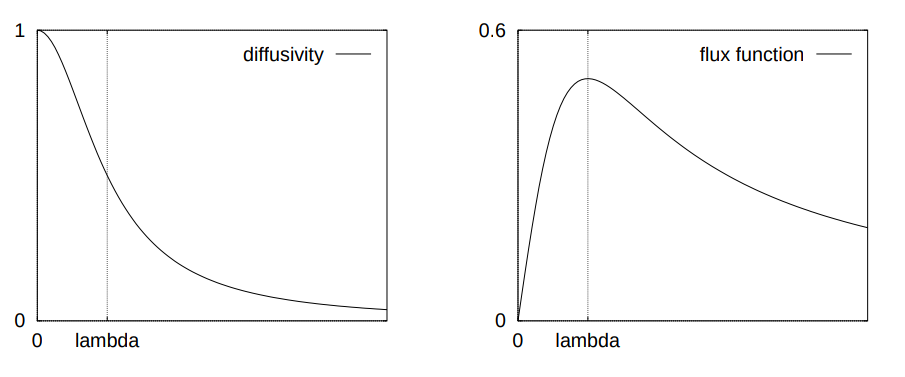
\includegraphics[width=\linewidth]{../Images/diffflux.png}
    \caption{\textbf{Left:} Diffusivity mentioned in~\eqref{def:Diffusivity}. \textbf{Right:} Flux
    function\eqref{def:Flux}. Source: \cite{dic18-04}}\label{fig:DiffFlux}
\end{figure}
As we already know, the flux describes the change in concentration at each position. The edge
enhancing effect comes from the so called \textit{backwards diffusion} which happens when the
gradient magnitude surpasses the contrast parameter as seen in \ref{fig:DiffFlux}. Backwards
diffusion is basically the opposite from `normal' diffusion in a sense that it sharpens image
features instead of smoothing them.
If we look at the derivative of the flux function this will become more obvious:
\begin{equation}
    \Phi'(s) = \frac{d}{ds} \left(\frac{s}{1 + s^2/\lambda^2}\right) = 
    \frac{1 - s^2/\lambda^2}{\left(1 + s^2/\lambda^2\right)^2}
\end{equation}
As we see, we have a maximum in the flux function at $s = \lambda$. Furthermore we can extract from
the above equation that $\Phi'(s) < 0$ for $s < \lambda$ and $\Phi'(s) > 0$ for $s > \lambda$. This
can also be seen in \ref{fig:DiffFlux}. This distinction between an increasing and decreasing flux
function for values left and right from the contrast parameter causes the previously mentioned
edge enhancing effect.
However, this particular process is not \textit{well-posed}\cite{weickert96}, i.e. it is very
sensitive to high frequent noise. To solve this, it was proposed to use Gaussian smoothing for
\textit{regularisation}, i.e. to convolve the original image with a Gaussian kernel to damp the high
frequencies that cause numerical instabilities\cite{catte-lions-morel92}.

\subsubsection{Nonlinear anisotropic diffusion}
But we can still go one step further and even make the direction of the smoothing process dependent
on the local structure. For example, one might want to prevent smoothing across edges and rather
smooth parallel to them further embracing the edge-preserving nature of nonlinear diffusion.

The diffusion tensor in this case is constructed from its eigenvectors $\boldsymbol v_1,
\boldsymbol v_2$ and eigenvalues $\lambda_1, \lambda_2$ using the
theorem of matrix diagonalisation
\begin{equation}
    \boldsymbol D = \left(\boldsymbol v_1\vert \boldsymbol v_2\right) \textnormal{diag}(\lambda_1, \lambda_2)
    \begin{pmatrix}
        \boldsymbol v_1^\top\\
        \boldsymbol v_2^\top
    \end{pmatrix}
\end{equation}
We define the the eigenvectors to be
\begin{align}
    \boldsymbol v_1 &\Vert \boldsymbol\nabla u_\sigma &\boldsymbol v_2 &\bot \boldsymbol\nabla
    u_\sigma
\intertext{As mentioned before, we want to encourage smoothing along edges and in flat regions. Thus, we
        define the eigenvalue for the eigenvector parallel to the gradient to be 1 and the eigenvalue to
        the orthogonal one to be a diffusivity function similar to the one in the nonlinear isotropic case.}
    \lambda_1 &= g(\lVert\boldsymbol\nabla u_\sigma\rVert_2^2) &\lambda_2 &= 1
\end{align}
There are different viable choices for a diffusivity function that supports backwards diffusion.
First, there is the already mentioned Perona-Malik diffusivity \eqref{def:Diffusivity}. Another
option is the diffusivity function introduced by Weickert\cite{weickert96}
\begin{equation}
    g(s^2) = \begin{cases}
        1 & s^2 = 0\\
        1 - \textnormal{exp}\left(\frac{-3.31488}{(s/\lambda)^8}\right) & s^2 > 0
    \end{cases}\label{def:WeickertDiff}
\end{equation}
According to \cite{dic18-04}, diffusivities of this type, i.e. rapidly decreasing diffusivities,
lead to more segmentation-like results.
Finally, the diffusivity that was mainly used for inpainting in this work is the
\textit{Charbonnier diffusivity} \cite{charbonnier}
\begin{equation}
    g(s^2) = \frac{1}{\sqrt{1 + s^2 / \lambda^2}}\label{def:CharbonnierDiff}
\end{equation}
\begin{figure}[ht]
    \centering
    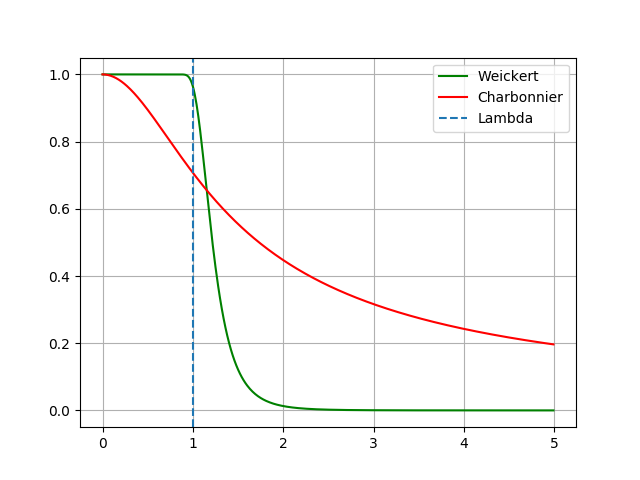
\includegraphics[width=\linewidth]{../Images/diffusivities.png}
    \caption{Weickert \eqref{def:WeickertDiff} and Charbonnier \eqref{def:CharbonnierDiff} diffusivities for $\lambda = 1$. Graph created with Matplotlib}
\end{figure}
\begin{figure}[ht]
    \centering
    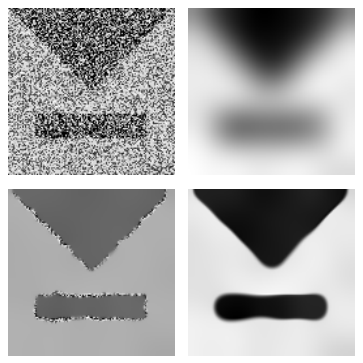
\includegraphics[width=0.8\linewidth]{../Images/diff_examples.png}
    \caption{Denoising capabilities of the different types of diffusion. \textbf{Top Left:} Original
    image. \textbf{Top Right:} Linear isotropic diffusion. \textbf{Bottom Left:} Nonlinear
isotropic diffusion. \textbf{Bottom Right:} Edge-enhancing diffusion. Source:
\cite{weickert96}}\label{fig:DiffExamples}
\end{figure}
%As we see in figure \ref{fig:DiffExamples}, EED possesses great restorative and denoising
%capabilities. But as Galić et al. showed, EED is also an excellent choice for
%PDE-based inpainting\cite{galic05}.
\section{EED-based inpainting}
Inpainting in digital image processing has first been introduced in \cite{bertalmio00}, as
mentioned in related work. They used 
\TODO{Shortly explain "normal" inpainting}
\TODO{Explain basics of EED inpainting}

\chapter{Numerical Aspects}\label{ch:Numerical} 
In this chapter, we will go over the numerical aspects of our work.
Firstly we are going to explain how images are usually defined in a discrete setting.
Afterwards, we will go over numerical differentiation and showcase how a so called
finite differences scheme for first order derivatives is derived. 
Lastly, we will talk about the discretisation of diffusion processes or, more specifically, the
discretisation of the EED process described in~\ref{sub:EEDInpaint}.
Since reality is not infinitely fine, things such as infinitesimal calculations as seen in 
calculus, e.g.\ differentiation of functions, can not be applied to the real world directly.
This is a problem since digital images are inherently not continuous as they contain only a
finite number of pixels. 

\section{Discrete Images}\label{sec:DiscreteImages}
Let $f:\Omega \rightarrow \R$ be an image where $\Omega
:= (0, n_x)\times(0, n_y) \subset \R^2$ as defined in Section~\ref{sec:Basics}. To
\textit{sample} the image, i.e.\ to discretise the image domain, we assume that all pixels lie on a
rectangular equidistant grid inside $\Omega$, where each cell in the grid has a size of $h_x
\times h_y$.
That yields $N_x := n_x/h_x$ pixels in x- and $N_y := n_y/h_y$ pixels in
y-direction.
That being said, we define the pixel $u_{i,j}$ at grid location ${(i, j)}^\top$ as
\begin{equation}
    u_{i, j} := u(ih_x, jh_y)\qquad \forall(i ,j) \in \{1,\dots,N_x\}\times\{1,\dots,N_y\}
\end{equation}
With that approach, the pixels are defined to lie on the crossing of the grid lines.
An alternative idea defines the pixels to lie in the centre of each cell, i.e.\ at location 
\begin{equation}
    {\left(\left(i-\frac{1}{2}\right)h_x,\ \left(j- \frac{1}{2}\right)h_y\right)}^\top
\end{equation}
As a sidenote, the cell sizes in either direction are almost always assumed to be 1 in 
practice. 
To keep the theory as universal as possible, however, we will use $h_x$ and $h_y$ instead.\\
Sampling of the spatial domain is not the only step necessary to fully discretise an image; we also have
to discretise the \textit{co-domain} or \textit{grey-value-domain}.\\
This step of the discretisation process is also called \textit{quantisation}.
In the continuous setting, the so called \textit{co-domain} is the complete set of irrational numbers $\R$.
To save disk space, this range is usually limited to 1 byte, that is values in the range 
of whole numbers from 0 to $2^8=256$~\cite{ipcv}.

\section{Numerical Differentiation}\label{sec:NumDiff}
Image derivatives are essential to image processing as seen in the previous chapter. 
Therefore, we need a way to compute them even on discrete images. To compute the 
gradient or, in the simpler case, the derivative of a discrete function, one 
generally uses so called \textit{finite difference schemes}. 
Such a scheme is normally derived from the \textit{Taylor expansion} of the continuous
function. For example, we want to compute the first derivative of a 1D function $f:\R
\rightarrow \R$, following closely the method described in~\cite{ipcv}.
The Taylor expansion of \textit{degree $n$} of this function around the point $x_0\in\R$ is given by 
\begin{equation}
    f(x) = T_n(x, x_0) + \mathcal{O}(h^{n+1})
\end{equation}
where $\mathcal{O}(h^{n+1})$ describes the magnitude of the leading error term and as such the
\textit{approximation quality} of the Taylor series.
The actual Taylor series is defined as
\begin{equation}
    T_n(x, x_0) = \sum\limits_{k=0}^{n} \frac{{(x-x_0)}^k}{k!}f^{(k)}(x_0)
\end{equation}
where $f^{(k)}$ denotes the $k$-th derivative of the function $f$.
A finite difference scheme generally uses a weighted sum of neighbouring values to compute the
desired derivative expression. In our example, we want to derive a scheme to compute the first
derivative of $f_i$ using its neighbours $f_{i-1}$ and $f_{i+1}$, i.e.
\begin{equation}
    f_i' \approx \alpha f_{i-1} + \beta f_i + \gamma f_{i+1}
\end{equation}
We can now describe $f_{i-1}$ and $f_{i+1}$ in terms of their Taylor expansion around $f_i$: 
\begin{align}
    f_{i-1} &= f((i-1)h) \notag\\
            &= T_n((i-1)h, ih) + \mathcal{O}(h^{n+1})\notag\\
            &= \sum\limits_{k=0}^{n}\frac{{(-h)}^k}{k!}f_i^{(k)}+ \mathcal{O}(h^{n+1})\\
    f_{i+1} &= \cdots = \sum\limits_{k=0}^{n}\frac{h^k}{k!}f_i^{(k)}+ \mathcal{O}(h^{n+1})
\end{align}
If we now choose a concrete value for $n$ (here $n=5$) we can actually compute the approximation:
\begin{align}
    f_{i-1} &= f_i - hf_i' + \frac{h^2}{2}f_i'' - \frac{h^3}{6}f_i^{(3)} + \frac{h^4}{24}f_i^{(4)} -
    \frac{h^5}{120}f_i^{(5)} + \mathcal{O}(h^6)\label{eq:fi-1}\\
    f_{i+1} &= f_i + hf_i' + \frac{h^2}{2}f_i'' + \frac{h^3}{6}f_i^{(3)} + \frac{h^4}{24}f_i^{(4)} +
    \frac{h^5}{120}f_i^{(5)} + \mathcal{O}(h^6)\label{eq:fi+1}
\end{align}
The next step is the \textit{comparison of coefficients}. We insert~\eqref{eq:fi-1} and~\eqref{eq:fi+1}
into the equation and solve the arising linear system of equations for $\alpha,\beta,\gamma$.
\begin{align}
    0\cdot f_i + 1\cdot f_i' + 0\cdot f_i'' \overset{!}{=} \alpha f_{i-1} + \beta f_i + \gamma
    f_{i+1}
\end{align}
After the substitution, the right hand side becomes
\begin{align}
    &\alpha \left(f_i - hf_i' + \frac{h^2}{2}f_i''\right) + \beta f_i + \gamma\left(f_i + hf_i' + \frac{h^2}{2}f_i''\right)\notag\\
    = &\left(\alpha+\beta+\gamma\right)f_i + h\left(-\alpha+\gamma\right)f_i' + \frac{h^2}{2}\left(\alpha+\gamma\right)f_i''
\end{align} 
Note that for the comparison of coefficients it suffices to use the first 3 summands of the
approximation. The linear system defined by the above equation
\begin{equation}
    \begin{pmatrix}
        1&1&1\\
        -1&0&1\\
        1&0&1
    \end{pmatrix}
    \begin{pmatrix}
        \alpha\\
        \beta\\
        \gamma
    \end{pmatrix}
    =
    \begin{pmatrix}
        0\\
        \frac{1}{h}\\
        0
    \end{pmatrix}
\end{equation}
has the solutions $\alpha = -\frac{1}{2h}, \beta = 0, \gamma = \frac{1}{2h}$.
This yields the approximation 
\begin{equation}
    f_i'\approx\frac{f_{i+1} - f_{i-1}}{2h}
\end{equation}
To find out how good this scheme is, we re-insert~\eqref{eq:fi-1} and~\eqref{eq:fi+1} to get
\begin{align}
    \frac{f_{i+1} - f_{i-1}}{2h}= -&\frac{1}{2h}\left(f_i - hf_i' + \frac{h^2}{2}f_i'' -
        \frac{h^3}{6}f_i^{(3)} + \frac{h^4}{24}f_i^{(4)} -
    \frac{h^5}{120}f_i^{(5)} + \mathcal{O}(h^6)\right) + \notag\\
                                   &\frac{1}{2h}\left(f_i - hf_i' + \frac{h^2}{2}f_i'' -
                                       \frac{h^3}{6}f_i^{(3)} + \frac{h^4}{24}f_i^{(4)} -
                                   \frac{h^5}{120}f_i^{(5)} + \mathcal{O}(h^6)\right)\notag
\end{align}
Expanding and simplifying yields
\begin{align}
        \frac{f_{i+1} - f_{i-1}}{2h} &= f_i' + \underbrace{\frac{h^2}{6}f_i'' +
            \frac{h^4}{30}f_i^{(4)} +
        \mathcal{O}(h^5)}_\text{quadratic leading error term}\notag\\
            \Rightarrow \frac{f_{i+1} - f_{i-1}}{2h} &= f_i' + \mathcal{O}(h^2)
\end{align}
This means that the error of our approximation is quadratic in the grid size. 
We also say that this approximation has a \textit{consistency order} of 2. Note that for such an
approximation to be reasonable, it has to have at least consistency order of 1. Otherwise, it is
not guaranteed that the error term diminishes if we send the grid size $h$ to 0.\\
The scheme derived above is also called \textit{central difference scheme}. Note that there are
other schemes such as \textit{forward} and \textit{backward} differences, but for the most part, we
will only use central differences since it provides us with the highest consistency
order out of all three. 
\begin{align}
    f_i' &= \frac{f_i - f_{i-1}}{h} + \mathcal{O}(h)&\textnormal{(backward differences)}\notag\\
    f_i' &= \frac{f_{i+1} - f_i}{h} + \mathcal{O}(h)&\textnormal{(forward differences)}\notag
\end{align}
\section{Numerical Schemes for Diffusion}\label{sec:NumSchemesDiffusion}
As discretisation for the inpainting process, the non-standard discretisation scheme as
derived in~\cite{www13} was used. The actual derivation of the scheme is fairly complex 
and beyond the scope of this thesis.
That is why we will just cover the essential information and then refer the interested 
reader to~\cite{weickert96, www13} for more information on numerical schemes for diffusion
processes in general.\\
We remember the defining equation of EED\@:
\begin{equation}
    \partial_t u = \diverg(\underbrace{g(\del\mathbf{u}_\sigma\del\mathbf{u}_\sigma^\top)}_{=:\mathbf{D}}\del
    \mathbf{u})\label{eq:EED}
\end{equation}
To discretise this equation, we first write the diffusion tensor $D$ as a symmetric matrix
\begin{equation}
    D = \begin{pmatrix}
        a&b\\b&c
    \end{pmatrix}
\end{equation}
Resubstituting this into~\eqref{eq:EED}, we get 
\begin{equation}
\partial_t u = \diverg \begin{pmatrix}
    a\cdot \partial_x u+b\cdot \partial_y u\\
    b\cdot \partial_x u+c\cdot \partial_y u
\end{pmatrix} = a\cdot\partial_{xx} u + 2b\cdot \partial_{xy}u+ c\cdot \partial_{yy} u
\end{equation}
These second order derivatives can easily be discretised using central differences. This leads to a
fairly complex stencil that the interested reader can look up in~\cite{weickert96}.
The problem with this discretisation is that it is not guaranteed to satisfy the
\textit{nonnegativity requirement} or \textit{stability in the maximum norm}~\cite{weickert96}. This requirement is
an important theoretical requirement as it is needed to guarantee the well-posedness of the
diffusion process, which in turn guarantees the numerical stability of the
algorithm~\cite{weickert96}.
In order to enable the discretisation to fulfill this requirement, one has to impose the restriction that
the \textit{spectral condition number $\kappa$}, which is the ratio between the smallest and
largest eigenvalue of the matrix $D$, is bounded by 
\begin{equation}
    \kappa \leq 3 + 2\sqrt{2}
\end{equation}
This restriction might seem arbitrary, but the proof of this upper bound can be found
in~\cite{weickert96}.
However, this requirement also puts a restriction on the anisotropy of the diffusion process, as the
ratio between the largest and smallest eigenvalue of the diffusion tensor is now bounded from above.
Therefore, one might consider another discretisation that is not necessarily stable in
the maximum norm.
In~\cite{www13}, Weickert et al.\ derived a framework for discretisations stable in the
\textit{Euclidean or 2-norm}. This framework embeds a series of 8 different
stencils. An example for such a stencil can be seen in Figure~\ref{fig:Stencil}.
\begin{figure}[ht]
    \centering
    \includegraphics[width=\linewidth]{Stencil}
    \caption{$L^2$-stable nonstandard stencil for anisotropic diffusion in dependence of parameters
    $\alpha, \beta$~\cite{www13}}\label{fig:Stencil}
\end{figure}
These stencils are dependent on 2 parameters $\alpha,\beta$ which can both be variant in space.
In the specific implementation we are using, $\alpha$ is fixed, while $\beta$ is space variant.
Additionally, a \textit{nonnegativity parameter} $\lambda \in [0,1]$ was introduced that is required
in the computation of the space-variant parameter $\beta$. \newpage\noindent
The parameter $\beta$ at location $(i,j)$ is then calculated as 
\begin{equation}\label{eq:Gamma}
    \beta_{i,j} = \gamma \cdot (1-2\alpha) \cdot \text{sgn}(b_{i,j})
\end{equation}
where sgn is the \textit{signum function} that returns the sign of a number
\begin{equation}
    \text{sgn}(x) = \begin{cases}
        0 & \text{ if } x = 0\\
        \dfrac{x}{\lvert x\rvert} & \text{ else }
    \end{cases}
\end{equation}
Let us now denote such a spatial discretisation of~\eqref{eq:EED} by 
\begin{equation}
    \frac{d\mathbf{u}}{dt} = \mathbf{A}(\mathbf{u})\mathbf{u}
\end{equation}
It can be shown that the matrix $\mathbf{A}$ is negative semidefinite, i.e.\  
\begin{equation*}
    x^\top \mathbf{A}x \leq 0
\end{equation*}
for all vectors $x$, if the parameters $\alpha,\beta$ satisfy
\begin{eqnarray}
    0 \leq \alpha \leq \frac{1}{2}\\
    \vert\beta\vert \leq 1-2\alpha
\end{eqnarray}
The negative semidefiniteness of $\mathbf{A}$ is useful to show that the semi-implicit and
explicit time discretisations both are stable in the 2-norm.\newpage\noindent
Both time discretisations work by applying a forward difference on
the temporal derivative on the left side with a time step size $\tau$ (this corresponds to the grid
size in the spatial derivative). 
The difference between the explicit and the implicit time discretisation is fairly small, but makes
a huge difference in efficiency since, as we will see next, we can choose much larger time steps in
the semi-implicit scheme than in the explicit scheme. 
The difference lies in the fact, that in the explicit scheme, the right hand side does not involve any terms
`from the future', while in the semi-implicit scheme it does.
We can now write the explicit scheme given by
\begin{equation}
    \frac{u^{k+1} - u^{k}}{\tau} = \mathbf{A}(u^k)u^k
\end{equation}
as
\begin{equation}
    u^{k+1} = (I + \tau\mathbf{A}(u^k))u^k
\end{equation}
The upper index $k$ denotes the `time level' of $u$.
Stability for this scheme can be guaranteed, if 
\begin{equation}
    \rho(I + \tau\mathbf{A}(u^k)) \leq 1\ \Leftrightarrow\ \tau \leq \frac{2}{\rho(\mathbf{A}(u^k))}
\end{equation}
where $\rho$ denotes the \textit{spectral norm} or \textit{modulus of the largest
eigenvalue}~\cite{www13}.
The semi-implicit scheme, however, is given by
\begin{equation}
    \frac{u^{k+1} - u^{k}}{\tau} = \mathbf{A}(u^k)u^{k+1}
\end{equation}
which boils down to solving the linear system of equations
\begin{equation}
    (I-\mathbf{A}(u^k))u^{k+1} = u^k\label{eq:SemiImpl}
\end{equation}
Note that the matrix on the left hand side is invertible thanks to the negative semidefiniteness of
$\mathbf{A}(u^k)$: One can show that because of the negative semidefiniteness, $(I-\mathbf{A}(u^k))$ only has eigenvalues
larger than 1.
This shows that the semi-implicit scheme given by 
\begin{equation}
    u^{k+1} = {(I- \mathbf{A}(u^k))}^{-1}u^k
\end{equation}
is stable in the 2-norm for every time step size $\tau$.\newpage\noindent
Furthermore, in the semi-implicit scheme the next iteration can not be computed explicitly (as the name
suggests) as is the case with the explicit scheme. Instead one has to solve
the linear system of equations given by~\eqref{eq:SemiImpl}. This is usually done with an iterative
solver like Gauss-Seidel or conjugate gradients (CG)~\cite{conjugateGradients}.\\
An in-depth explanation of these solvers would be beyond the scope of this thesis.
Hence, the only thing important to know is that for the evaluation of the inpainting masks in our work,
we used a semi-implicit scheme with a CG solver and a timestep size of 1000.
Moreover, we implemented a stopping criterion which ensures that the residual error of the solution
of the CG solver is below a set threshold of $10^{-6}$.

\chapter{Corner Regions and Additional Procedures}\label{ch:Modelling}
In this chapter we will introduce corner regions as an essential concept of this work and talk
about the additions we made to the corner detection algorithm in order to select the most valuable
corners for our inpainting mask.\\
The initial corner detection algorithm as well as the code for the inpainting algorithm was given
to me by courtesy of Joachim Weickert.

\section{Disk-shaped Corner Regions}
As mentioned in the beginning, the main concern for the approach of Zimmer~\cite{zimmer07}, alongside 
MCM not being suitable for inpainting, was that the corner localisation was not accurate enough that 
We can just keep a 4 or 8-neighbourhood of pixels.
The implication is that the regions he inserted into the mask were were too small to
cover the potential uncertainty in the corner localisation process stemming from the Gaussian
smoothing in the computation of the structure tensor (see Section~\ref{sec:Structure}). Specifically
because in order to limit the amount of corners detected, Zimmer chose to vary the integration scale
parameter increasing the uncertainty in the localisation, this poses a problem.
Hence, we want to explore increasing the neighbourhood of pixels that is kept around each
corner. A disk-shaped neighbourhood or \textit{(disk-shaped) corner region} with radius $r$ and origin point $(x, y)$ is defined as 
\begin{equation}
    B_r(x, y) = \lbrace (x',y') \in \Omega\ \vert\ {(x'-x)}^2 + {(y'-y)}^2 \leq r^2\rbrace
\end{equation}
The optimal choice for the radius of the corner disks is discussed in
Section~\ref{sec:ParameterSelection}.
Increasing the radius of the corner regions obviously leads to denser masks if one does not adjust
the limit of corner regions that are put in the mask. Since doing this manually for every picture
would not be practical at all in the context of a codec, we have to come up with a way to make sure
the resulting masks are always similar in pixel density.\newpage\noindent
One way to achieve this would be to introduce a percentile parameter instead of using the constant
threshold from the corner detection method described in~\ref{sub:Corner}.

\section{Percentile Thresholding}\label{sec:Percentile}
In the classic version of Harris corner detection, an artificial threshold parameter $T$
is introduced to weed out `bad' corners, i.e.\ corners where the \linebreak 
Harris measure~\eqref{def:Harris} is low. 
This parameter, however, is fairly sensible to the input image.\\
As a workaround to make this parameter a bit more robust, a percentile
parameter is introduced that is in turn used to compute a more robust threshold.\\
In statistics, the \textit{n-th percentile} of a set is the value that is larger than $n$ percent
of all values in this set.
We computed the percentile using the \textit{nearest-rank method} since this was the easiest
approach and worked good enough already. In this method, the n-th percentile is just simply
computed as the value at position 
\begin{equation} 
    \left\lceil \frac{n}{100}\cdot N_{x}N_{y}\right\rceil 
\end{equation} 
of the ordered set of values~\cite{percentile}.\\
Since in an image, there are more non-corners than actual corners, we have to deal with many zero
or close-to-zero cornerness values. This is a problem because the percentile computation would be skewed
heavily if e.g.\ more than 80 percent of all values are zero already. To solve this, we first filtered
out all values below a threshold close to zero and then accumulated the remaining values into an
array of appropriate size. This array is then sorted using an already implemented Quicksort
algorithm from the C standard library.\\
Subsequently, the new threshold is given as the value at the index calculated above.
While this approach works a bit better than the original version using the fixed threshold, it is
still not perfect. For example, if one uses a percentile of $0.5$, meaning that 
$50\%$ of all corners are thrown out, one could still get wildly different results 
for two different input images as we can see in~\ref{fig:PercExample}.
\begin{figure}[h!]
    \centering
    
\includegraphics[width=0.4\linewidth]{example_rect_50.png}
    
\includegraphics[width=0.4\linewidth]{example_cat_50.png}
    \caption{Corner detection with the same parameters. Parameters are $\sigma=1,\rho=2,q=0.3$, no
    CNMS, no TPPT}\label{fig:PercExample}
\end{figure}\\
To tackle this issue, we propose a new method that we call \textit{Total Pixel Percentage
Thresholding}. The idea behind this method is that one makes the amount of corners that are kept
in the masks dependent on the mask radius, i.e.\ the radius of a corner region in the inpainting
mask.\newpage\noindent
In other words, one specifies the desired mask pixel density and depending on the mask
radius, the maximum number of corners that can be inserted into the mask is
calculated.
The problem of calculating the number of pixels inside a disc of radius $r$ is also known as
\textit{Gauss' circle problem}~\cite{gaussCircle}. The exact solution to this problem is given
by~\cite{hilbert96}
\begin{equation}
    N(r) = 1 + 4\sum_{i=0}^{\infty}\left(\left\lfloor\frac{r^2}{4i+1}\right\rfloor - \left\lfloor
    \frac{r^2}{4i+3}\right\rfloor\right)
\end{equation}
but since this is an infinite sum, the exact solution can not be computed this way. This is why we
chose the naive way by just iterating through a loop and count the pixels inside the disk.
We could have also chosen to use an upper bound and estimate the number of pixels that 
way, but this would not have been as accurate.\\
After computing the area occupied by a single corner region we can simply calculate an upper bound on the number of
regions that can be inserted into the mask without exceeding the pixel density threshold by the equation
\begin{equation}
    N_{corners} = \left\lceil \frac{q \cdot N_{x}N_{y}}{N_{disc}} \right\rceil,\qquad0\leq q\leq 1 
\end{equation}
where $q$ is the percentile parameter, $N_x, N_y$ the number of pixels in the respective direction
and $N_{disc}$ the amount of pixels per corner region. 
Using this method, the pixel density of inpainting masks can be consistently recreated, as we will
see in the next chapter where we will present some examples of this method in
action.\newpage\noindent
Note that we did not consider the potential overlap of corner regions inside the
computation of $N_{disc}$, which is why this is only an upper bound, since there would have been no 
easy way to determine the amount of overlapping pixels a priori.\\
Instead, we introduced another method tackling the issue of potentially overlapping corner regions
called \textit{Circular Non-Maximum Suppression}. We will see how this method
works in the next Section~\ref{sec:Suppression}.
Another noteworthy point is that the amount of pixels in the mask using this approach is limited by
the number of corners detected since we do not even consider pixels that have a sufficiently small
cornerness value as mask candidates.
\section{Circular Non Maximum Suppression}\label{sec:Suppression}
\begin{figure}[t]
    \begin{lstlisting}[language=Python]
# Circular non-maximum suppression at x with radius r.
# Parameters:
#    -harris: Harris measure map
#    -x: current location as tuple
#    -r: radius of corner regions
#    -out: map of accepted corners after suppression
def circular_suppression(harris, x, r, out):
    for y in circle(x, r):
        if harris[y] > harris[x]:
            # The current location is not a maximum
            out[x] = 0
            return
    # Current location is a maximum, keep the region around it
    out[x] = harris[x]
    \end{lstlisting}
    \caption{Pseudo-Code for circular non-maximum suppression}
\end{figure}
\noindent As mentioned previously, overlapping corner regions tend to worsen the estimation of the mask pixel
density. 
Furthermore, as Zimmer~\cite{zimmer07} already stated, the sparsity of corners in images poses a
problem for the reconstruction quality. Circular non-maximum suppression is supposed to tackle both of these 
issues by increasing the radius of the local maximum search during the corner detection. 
In the original corner detection method, corners are determined by the local maxima inside an 
8-neighbourhood of the cornerness measure. The idea is to adapt the radius of the neighbourhood for the
local maximum search to the mask radius.\newpage\noindent
As experiments showed (see Section~\ref{sec:Results}), this minimises the overlap in
corner regions in the final mask and enables a fairly accurate estimation of the mask pixel
density, allowing us to consistently produce masks with similar density.
The other issue that this method tries to solve is the uneven distribution of corners across
the whole image. When limiting the amount of corners that are selected as candidates for the mask, one should not only care about
the `cornerness' of a corner, but also about its position. 
In other words, if a lot of good corners
are in close proximity to each other, it would be better to choose the ones that encase the 
highest number of `good' corners around them. 
That way, we get multiple corners `for the price of one' and can still introduce some 
of the `worse' corners to the mask.
By minimising the overlap between corner regions through this circular non-maximum suppression, we
can actually eliminate corners that are already covered by another disk from `a better' corner and
thus free up some slots for corners that may otherwise not have been selected for being sub-par.\\
One should note that this is not a perfect solution as certain constellations of corners create
an edge case in which a corner that is assumed to cover another corner is removed for being in the
disk of a better corner. This leads to the case where the corner that was formerly assumed to be
covered is suddenly not covered anymore and disappears from the mask without replacement, so future
work might be invested into finding a better solution for this approach.


\chapter{Experiments}\label{ch:Experiments} 
In this chapter, we will focus on some experiments that we performed and their results.
In the first part, we show the images that were used for the experiments. Afterwards we are going
to tackle the point of parameter selection since it is not trivial to find the optimal set of
parameters. Therein, we explain the meaning of each parameter in both the corner detection and
inpainting process as well as present a reasonable choice for them.
Lastly, we present some results from the experiments and whether or how this is useful for
PDE-based image compression methods.
\section{Test images}
We divide the test images in 2 different groups because as we will see later in this chapter, the
method works better on a certain category of images.
First, we have the `normal' grey value images as seen in figure \ref{fig:GreyValueImg}. All these
images were provided by Joachim Weickert and count to the standard test images in the image
processing community.
The second groud is the group of binary grey value images, i.e. images that contain only black and
white pixels instead of 256 different grey values as is the case in the first category. Of this
second category (cf. figure \ref{fig:BinaryImg}), only the picture \texttt{cat} was provided by
Joachim Weickert, the other ones were generated by me using the image manipulation programme
\texttt{GIMP}. Each of these generated pictures was created to test or highlight different aspects
of the corner detection or inpainting method as seen in section \ref{sec:Results}.
\begin{figure}[ht]
    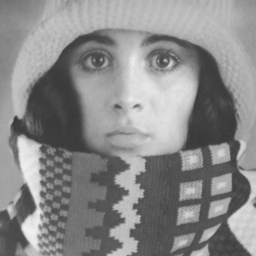
\includegraphics[width=0.5\linewidth]{../../images/grey/trui.png}
    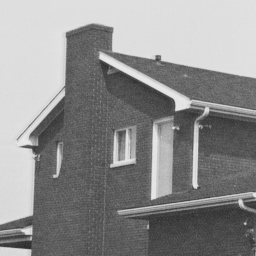
\includegraphics[width=0.5\linewidth]{../../images/grey/house.png}
    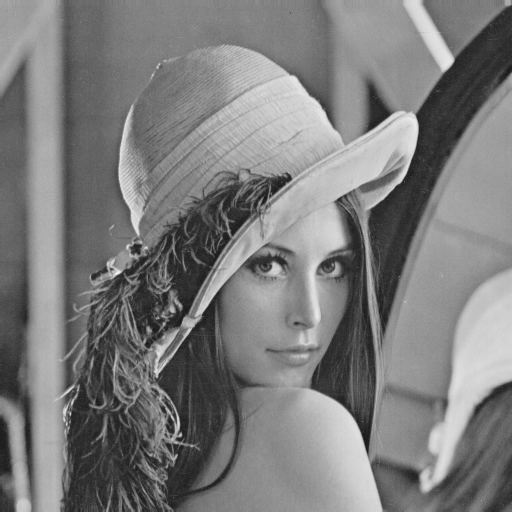
\includegraphics[width=0.5\linewidth]{../../images/grey/lena512.png}
    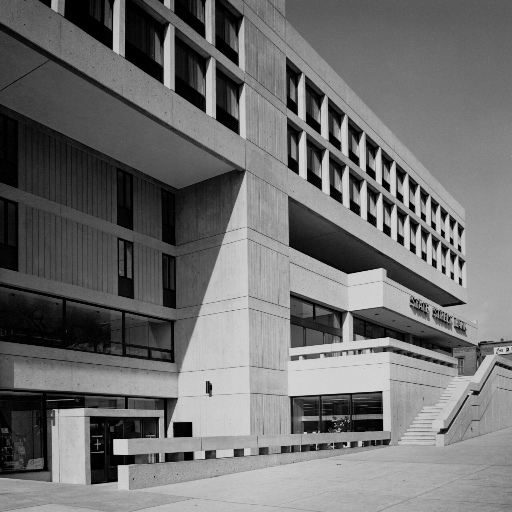
\includegraphics[width=0.5\linewidth]{../../images/grey/bank.png}
    \caption{Grey value images used for testing. From left to right and from top to bottom: \texttt{trui},
    \texttt{house}, \texttt{lena512}, \texttt{bank}}\label{fig:GreyValueImg}
\end{figure}
\begin{figure}[ht]
    
\includegraphics[width=0.32\linewidth]{../../images/binary/cat.png}
    
\includegraphics[width=0.32\linewidth]{../../images/binary/rect.png}
    
\includegraphics[width=0.32\linewidth]{../../images/binary/semicircle.png}
    
\includegraphics[width=0.32\linewidth]{../../images/binary/ellipse.png}
    
\includegraphics[width=0.32\linewidth]{../../images/binary/abstract1.png}
    
\includegraphics[width=0.32\linewidth]{../../images/binary/checkerboard32.png}
    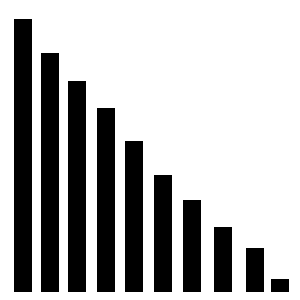
\includegraphics[width=0.32\linewidth]{../../images/binary/testlength.png}
    \caption{Binary images used for testing. From left to right and from top to bottom:
        \texttt{cat}, \texttt{rect},
    \texttt{semicircle}, \texttt{ellipse}, \texttt{abstract1}, \texttt{checkerboard32},
\texttt{testlength}}\label{fig:BinaryImg}
\end{figure}
\section{Parameter Selection}
As mentioned earlier, the optimal set of parameters is difficult to choose, that is why we have to
experiment a lot to find a decent approximation to this optimal set. In the following we will
therefore explain what the different parameters do, how that influences the image or mask quality
and ultimately, how we chose the parameters that we used to get our results.
First off, we talk about corner detection as this was the primary focus of our work. The parameter
choice was mainly fixed from the beginning as we used sets of parameters proven to be fairly
optimal in previous work by {<insert reference here>}. Nonetheless, we shortly go over the different
parameters and explain their influence.
\subsection{Corner Detection}
For corner detection there are not that many different parameters to play around with. In the
classical approach using the structure tensor (cf section \ref{sub:Corner}) we have only 3
parameters:
\begin{itemize}
    \item the noise scale $\sigma$
    \item the integration scale $\rho$ and
    \item a threshold parameter $T$ to filter out non-important corners
\end{itemize}
but as mentioned in section \ref{sec:Contribution}, we replaced the threshold by a percentile
parameter to make it more robust.
However, we introduced a new parameter $R$, that determines the size of the corner regions and
subsequently also the size of the region where the non-maximum suppression is performed in.

Regarding the noise scale, we generally want to choose it as large as necessary but keep it as small as
possible, meaning that we want to choose the smallest noise scale that gets rid of most of the
noise in the image since with a larger $\sigma$ 
one often faces the problem that the detected corners can not be located as accurately anymore,
since more and more relevant features are smoothed away (cf. scale space section). Another problem
is that the gaussian scale space (iterated gaussian smoothing) may even introduce new
corners.\cite{weickert96}
 Most of the time however, a $\sigma$ of 1 is sufficient enough to remove most of the noise and unnecessary
 details and still provide an accurate result.\\
Twe integration scale $\rho$ basically determines how `local' 
the corner detection is as it influences the size of the region structural information is averaged
in during the computation of the structure tensor. $\rho$ should always be chosen larger than the noise
scale $\sigma$, which leads us to a `standard' value of 2-2.5. In our experiments, these values
usually yielded the best results.\\
The newly introduced percentile parameter regulates the amount of corners that are ultimately being
detected since the percentile thresholding is applied \textit{after} the CNMS. 

\subsection{Inpainting}
The main parameters required by the inpainting process are 
\begin{itemize}
    \item the noise scale $\sigma$,
    \item the integration scale $\rho$,
    \item the contrast parameter $\lambda$, 
    \item the dissipativity parameter $\alpha$ and
    \item a non-negativity parameter $\gamma$.
\end{itemize}
The implementation of the algorithm that was provided by Joachim Weickert also requires some
technical parameters such as the choice of diffusivity function, time discretisation scheme, time
step size and iterative solver used for the semi-implicit time discretisation scheme.
 All these paramters were fixed beforehand. We used the Charbonnier diffusivity function mentioned
 in <theory>. As the other parameters are concerned, a semi-implicit scheme with a time step size
 of 1000 has been used. As an iterative solver for the system of equations that arises from the
 semi-implicit scheme a conjugate gradient solver with 200 iterations was used.
\\
If we recall from the theory section, when using EED, we do not need the integation scale, as the
integration scale only influences the radius of the structure tensor which is actually not needed
for this method of inpainting. Thus, this parameter will be fixed to 0.\\
The parameters $\alpha$ and $\gamma$ are purely numerical parameters that are used to 
stabilise the algorithm or rather help to ensure that the stencil weights of the discretisation of
the diffusion process meet certain requirements. A fairly optimal choice for these parameters has
been proposed in \cite{www13}, namely $\alpha=0.44, \gamma=0.98$.
In general, one could image the parameter $\alpha$ as a sharpness parameter: the larger the
$\alpha$ (but not larger than 0.5), the sharper the image. More on the nature of these two parameters can be read about in
\cite{www13, weickert96}.\\
Next up is the contrast parameter $\gamma$ that is required in the diffusivity function
\eqref{def:Diffusivity}. As already explained in the \ref{sec:Structure}, this parameter helps to
distinguish between edges and non-edges. For the EED inpainting this is especially important since
it basically determines how strongly edges will be continued into inpainting regions. We
experimented with different choices for this parameter but came to the conclusion that a fairly
small value yields the best results. In general, we used a value of 0.03 for most of the images,
but found that for a certain set of images, an even smaller value of 0.01 yielded better results.\\
Last but not least, the noise scale $\sigma$ determines how much the initial image is smoothed
before the computation of the image derivatives. In general, this parameter is always fixed at 1.0
as it only serves to regularise the differentiation process.
\section{Results}\label{sec:Results}

\chapter{Conclusion and Outlook}

\label{ch:Conclusion}

\section{What works well}
\section{What does not}
\section{Future Work}


%----------------------------------------------------------------------------------------
%   THESIS CONTENT - APPENDICES
%----------------------------------------------------------------------------------------

\appendix % Cue to tell LaTeX that the following "chapters" are Appendices

%----------------------------------------------------------------------------------------
%   BIBLIOGRAPHY
%----------------------------------------------------------------------------------------

\printbibliography

%----------------------------------------------------------------------------------------

\end{document}
